% 1.4.Solution.tex
%	Last update: 2019/07/24 F.Kanehori
%\newpage
\subsection{対処法}
\label{subsec:Solution}

\noindent
前節で示した問題点への対処法について述べます。

\bigskip
\noindent
\bf{ソースファイルの整合性}
\begin{narrow}[20pt]
	\SprLib のソースツリーにあるプロジェクトディレクトリ
	(\tt{Base}, \tt{Collision}, $\ldots$)を
	直接\tt{add\_subdirectory}すれば問題ありません。
\end{narrow}

\medskip
\noindent
\bf{ビルドの最適性(無駄なコンパイル)}
\begin{narrow}[20pt]
	\SprLib, \it{App1, App2\,}などのすべてで、
	ライブラリのオブジェクトが生成される場所を共通化してしまうことで
	この問題を回避することとします。
	具体的には、\SprLib ソースツリーの中(ビルドツリーの外)に
	オブジェクトの共通格納場所を作り、
	\SprLib およびすべてのアプリケーションでオブジェクト格納領域が
	そこを指すようにlinkを張ることとします。

\ifLwarp
	\begin{figure}[h]
	    \begin{center}
	    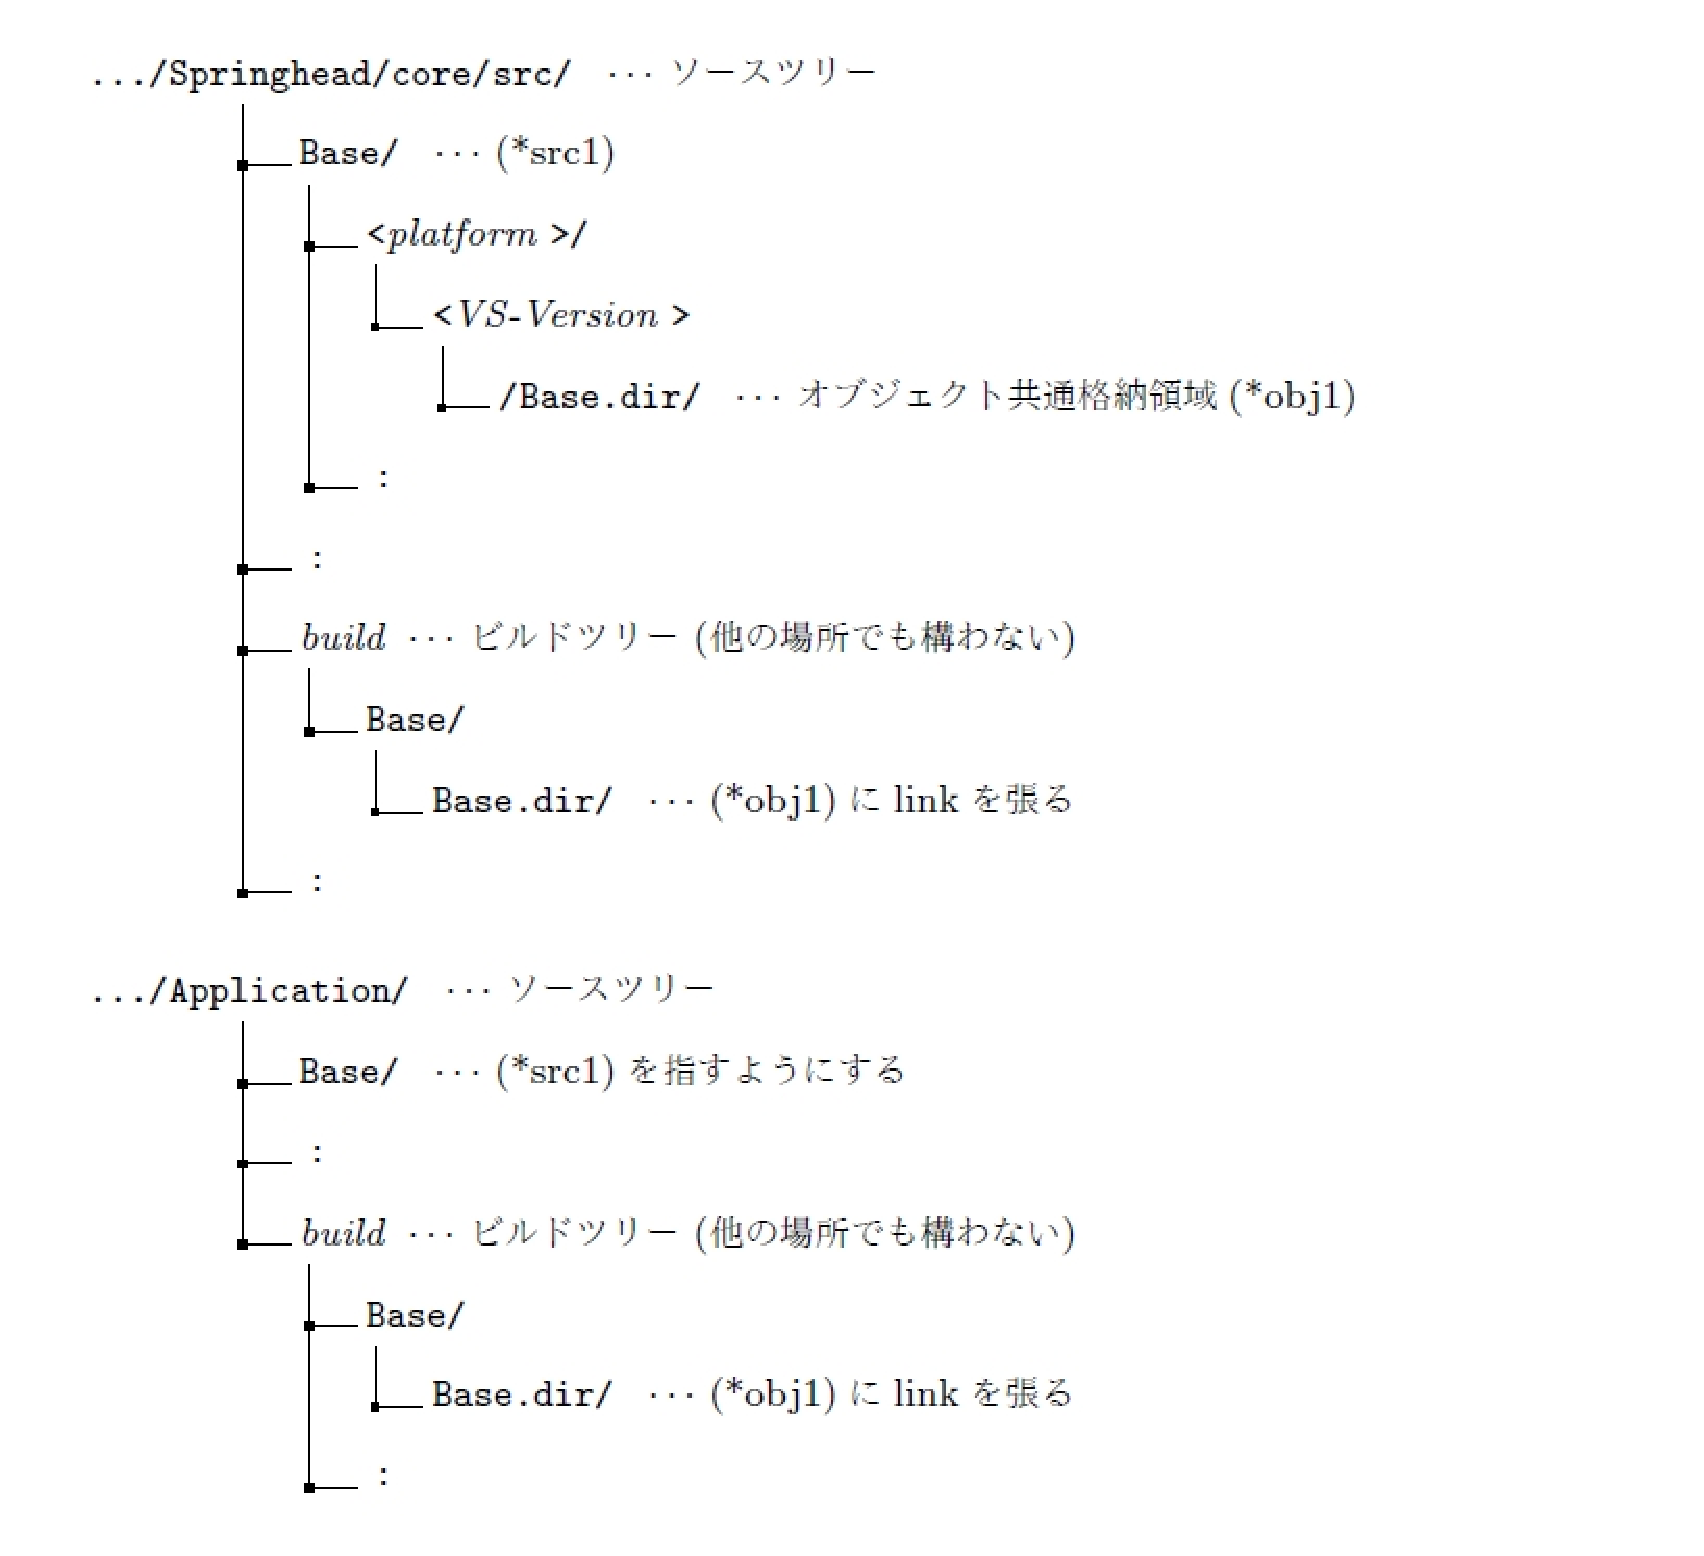
\includegraphics[width=.9\textwidth]{fig/ApproachToBuildOptimization.eps}
	    \end{center}
	    \caption{ビルドの最適性への対処法}
	    \label{fig:ApproachToBuildOptimization}
	\end{figure}
\else
	\begin{figure}[h]
    	\begin{narrow}[40pt]\begin{minipage}{\textwidth}
		{\footnotesize{\dirtree{%
			.1 \hspace{-10mm}.../Springhead/core/src/ \Anno{ソースツリー}.
			.2 Base/ \Anno{(*s1)}.
			.3 <\it{platform\,}>/.
			.4 <\it{VS-Version\,}>.
			.5 /Base.dir/ \Anno{オブジェクト共通格納領域(*o1)}.
			.3 :.
			.2 :.
			.2 \build \Anno{ビルドツリー (他の場所でも構わない)}.
			.3 Base/.
			.4 Base.dir/ \Anno{(*o1)にlinkを張る}.
			.2 :.
		}}}
		\medskip
    	\end{minipage}\end{narrow}
    	\begin{narrow}[40pt]\begin{minipage}{\textwidth}
		{\footnotesize{\dirtree{%
			.1 \hspace{-10mm}.../Application/ \Anno{ソースツリー}.
			.2 Base/ \Anno{(*s1)を指すようにする}.
			.2 :.
			.2 \build \Anno{ビルドツリー (他の場所でも構わない)}.
			.3 Base/.
			.4 Base.dir/ \Anno{(*o1)にlinkを張る}.
			.3 :.
		}}}
		\medskip
  	\end{minipage}\end{narrow}
	\caption{ビルドの最適性への対処法}
	\label{fig:ApproachToBuildOptimization}
	\end{figure}
\fi
	\indent
	このlinkを張る作業は、
	アプリケーションの\cmake\ (configure)時に行なうものとします。
\end{narrow}

\medskip
\noindent
\bf{プロジェクトファイルの整合性}
\begin{narrow}[20pt]
	ビルドの最適性の場合と同様、
	プロジェクトファイルも共通化することでこの問題に対処します。
	具体的には、各プロジェクトファイルは
	\SprLib ビルドツリーにあるものを共通に参照すべきファイルとし、
	すべてのアプリケーションのプロジェクトファイルは、そこへのlinkとします。

	 ただしこれでは不完全で、\App{1}で実施したプロジェクトファイルへの変更が
	\App{2}に伝わりません。
	このため\App{1}でプロジェクトファイルを変更した場合には、
	その変更を\SprLib ビルドツリーにあるプロジェクトファイルに反映させるものとします。
	つまり、\SprLib のビルドツリーにあるプロジェクトファイルを
	常に最新の状態に保つということです。

	 この作業はアプリケーションのビルド時に行なうものとします。
	そのために、各アプリケーションのソリューションファイルに
	特別なターゲット\tt{sync}を作成し、
	このターゲットが毎回のビルドに先立って実行されるようにします。

\ifLwarp
	\begin{figure}[h]
	    \begin{center}
	    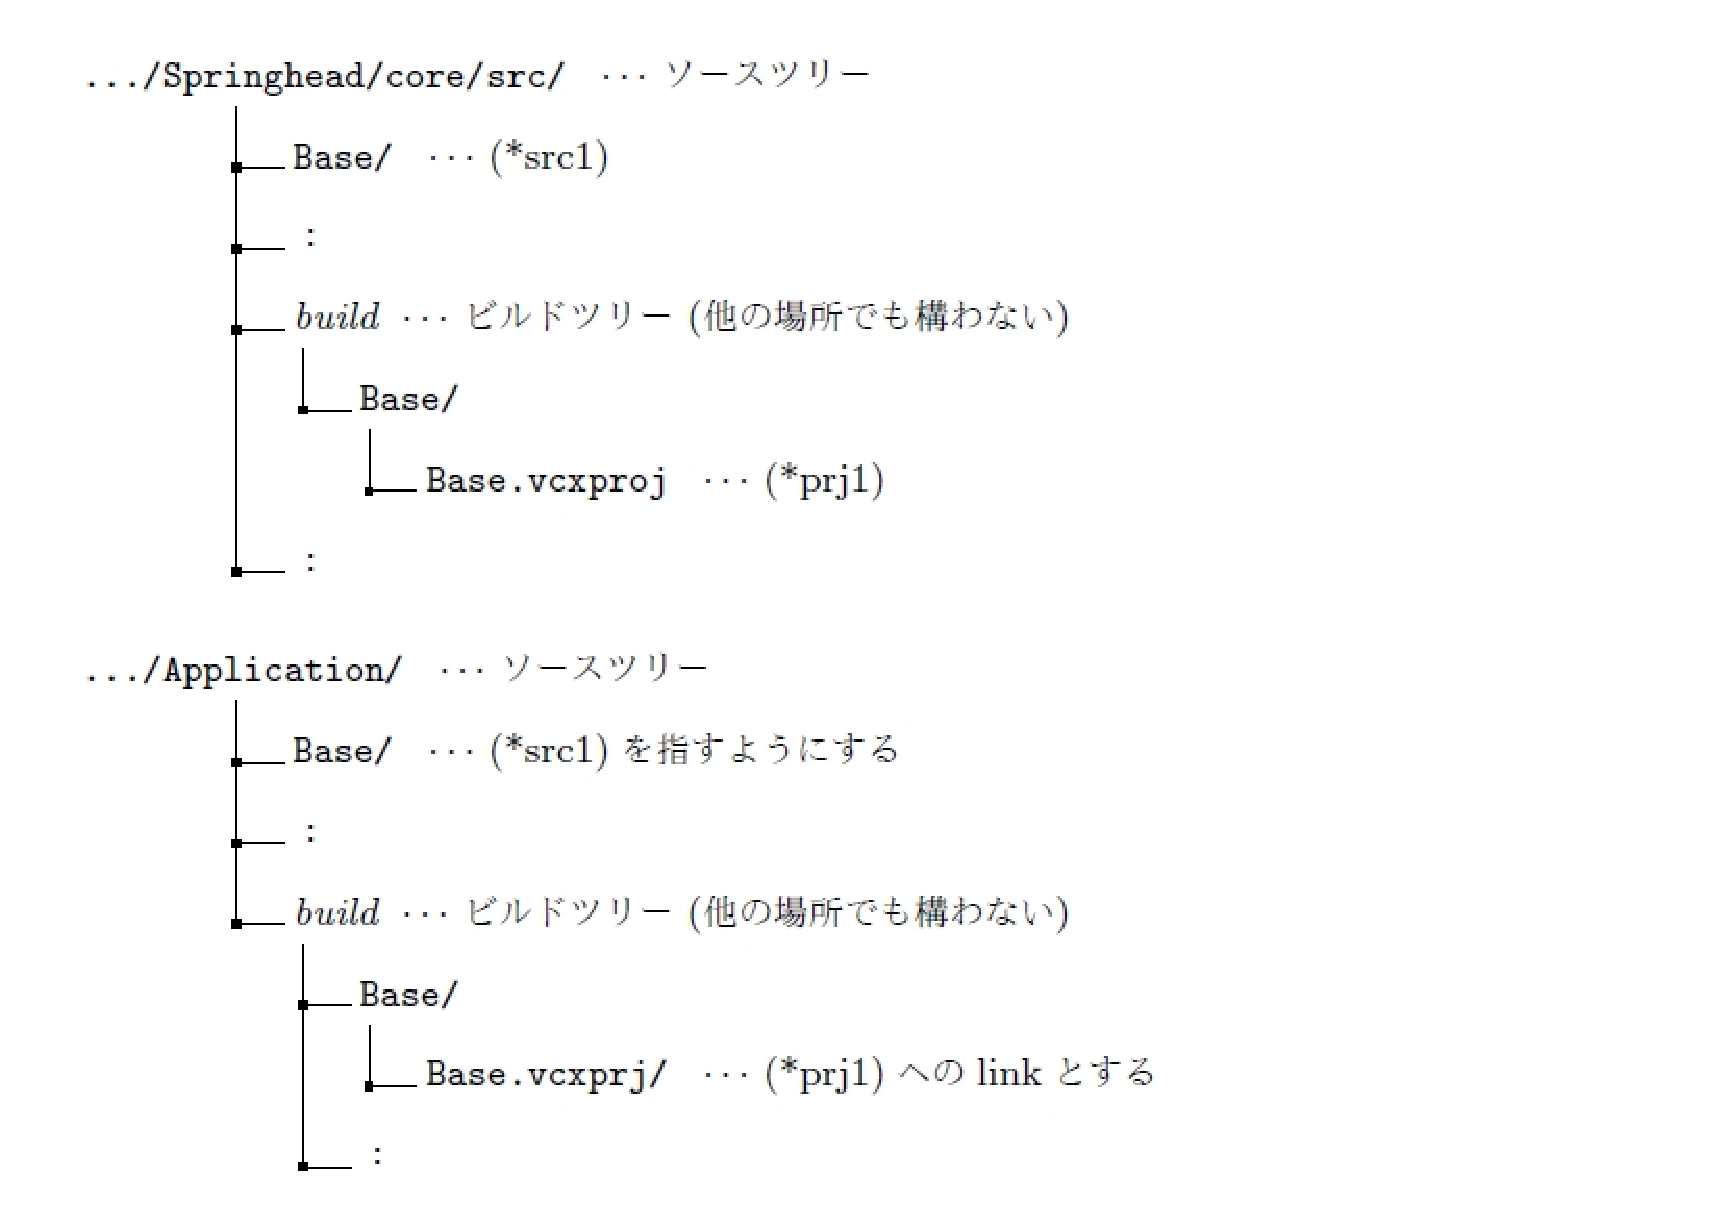
\includegraphics[width=.9\textwidth]{fig/ApproachToProjfileOptimization.eps}
	    \end{center}
	    \caption{プロジェクトファイルの最適性への対処法}
	    \label{fig:ApproachToProjfileOptimization}
	\end{figure}
\else
	\begin{figure}[h]
    	\begin{narrow}[40pt]\begin{minipage}{\textwidth}
		{\footnotesize{\dirtree{%
			.1 \hspace{-10mm}.../Springhead/core/src/ \Anno{ソースツリー}.
			.2 Base/ \Anno{(*s1)}.
			.2 :.
			.2 \build \Anno{ビルドツリー (他の場所でも構わない)}.
			.3 Base/.
			.4 Base.vcxproj \Anno{(*p1)}.
			.2 :.
		}}}
		\medskip
    	\end{minipage}\end{narrow}
    	\begin{narrow}[40pt]\begin{minipage}{\textwidth}
		{\footnotesize{\dirtree{%
			.1 \hspace{-10mm}.../Application/ \Anno{ソースツリー}.
			.2 Base/ \Anno{(*s1)を指すようにする}.
			.2 :.
			.2 \build \Anno{ビルドツリー (他の場所でも構わない)}.
			.3 Base/.
			.4 Base.vcxprj/ \Anno{(*p1)へのlinkとする}.
			.3 :.
		}}}
		\medskip
  	\end{minipage}\end{narrow}
	\caption{プロジェクトファイルの最適性への対処法}
	\label{fig:ApproachToProjfileOptimization}
	\end{figure}
\fi
	\indent
	
\end{narrow}

% end: 1.4.Solution.tex
